\chapter{Wstęp} \label{ch:introduction}

\section{Problem}

Celem tej pracy jest stworzenie systemu plików z mechanizmem
\textbf{Quality of Service (QoS)}, który będzie kształtował i ograniczał przepustowość dysku oraz pozwoli na zapewnienie sprawiedliwego względgem szybkości
dostępu do zasobów dyskowych.

\section{Cel badawczy}

Praca niniejsza ma na celu implementację mechanizmu \textbf{QoS} w systemie przechowywania danych,
pozwalającej na kontrolowanie szybkości transferu danych odczytu i zapisu operacji I/O.

Tego typu system taki mógłby być przydatny np. w strumieniowaniu dużych plików multimedialnych dla wielu klientów.
Zapewnienie minimalnej szybkości transferu danych podczas odczytu plików może znacząco podnieść wydajność
takich usług.

\subsection{Cel praktyczny}
Zaimplementowany zostanie system plików o nazwie \textbf{QoSFS}\footnote{Quality of Service Filesystem}, który pozwoli na ustalanie minimalnej potrzebnej szybkości transferu danych do wykonywania operacji I/O.

\subsection{Cel teoretyczny}
Teoretyczna część pracy zawiera analizę wykonanego systemu pod kątem przydatności,
opóźnień odczytu i zapisu oraz ewentualnych przeciążeń w komunikacji.
W tym celu stworzone zostana odpowiednie benchmarki wykonujące operacje na plikach,
które umożliwiają analizę zaimplementowanego rozwiązania.

\section{Struktura pracy}

\begin{itemize}
  \item Rozdział \textbf{\ref{ch:introduction}}
	opisuje postawione cele - teoretyczny i praktyczny oraz zawiera opis struktury pracy.

	\item W rozdziale \textbf{\ref{ch:subject-introduction}} znajduje się
	wprowadzenie do tematyki pracy oraz opis wykorzystanych technologii. 
	Wytłumaczono jak działa wirtualny system plików, opisano
    ideę systemu plików w przestrzeni użytkownika i wybraną metodę
    testowania zaimplementowanego rozwiązania.

	\item Rozdział \textbf{\ref{ch:articles}} przeznaczony jest na przegląd
    artykułów, które zostały wykorzystane podczas pracy.
    
    \item W rozdziale \textbf{\ref{ch:prototypes}} opisano wszystkie rozważane rozwiązania,
    które nie znalazły się w pracy oraz wytłumaczono powody, dla których
    z nich zrezygnowano.
    
    \item Projekt oraz implementacja systemu zostały przedstawione w rozdziale \textbf{\ref{ch:implementation}}.
    Znajduje się tam projekt modelu systemu oraz dokładny opis każdego
    z modułów oraz sposobu ich testowania.
    
    Dodatkowo można tam znaleźć instrukcję użytkownika (instalacja i uruchomienie systemu)
    oraz narzędzia użyte podczas procesu implementacji.
    
    \item W rozdziale \textbf{\ref{ch:experiments}} scharakteryzowano
    system, na którym przeprowadzono testy i przedstawiono wyniki
    oraz ich analizę.
    
    \item Ostatni rozdział \textbf{\ref{ch:summary}} poświęcony jest na
	wnioski oraz prezentację możliwych kierunków rozwoju systemu.
    
    \item W końcowej części pracy znajduje się bibliografia.
\end{itemize}

\chapter{Wprowadzenie do tematyki} \label{ch:subject-introduction}

Aby sprostać wymaganiom stawianym przez rozwój technologiczny, systemy przechowywania
danych z roku na rok stają się coraz pojemniejsze i szybsze. W porównaniu z pierwszym dyskiem twardym, który mógł przechowywać zaledwie 5MB danych, aktualna standardowa pojemność dysków jest
mniej wiecej 200,000 razy wieksza.

\begin{figure}[h!]
	\centering
	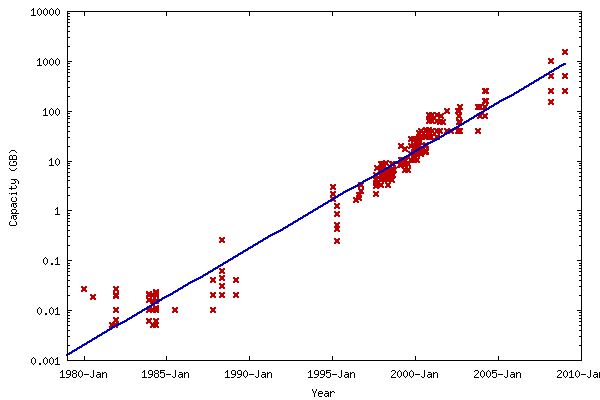
\includegraphics[scale=0.5]{HDDOverTime.png}
		\caption{Zmiana pojemności dysków na przestrzeni lat}
\end{figure}

Ponadto, przechowywane dane należą do różnych typów, z których wiele może mieć narzucone pewne wymagania
szybkości transferu danych. Na przykład, gdy otwieranie dużego pliku tekstowego zajmuje kilka lub
kilkanaście minut, nie jest to tak uciążliwe jak kilkusekundowe wczytywanie każdej klatki
pliku multimedialnego.

Quality of Service jest używany głównie w telekomunikacji, gdzie administratorzy
sieci mogą go używać do zapewnienia przepustowości dla krytycznych aplikacji aby ich transakcje zostały przetworzone w akceptowalnym czasie.

\section{Virtual File System}
System będzie działać w oparciu o
\textbf{VFS (Virtual File System)} w systemie Linux. VFS jest abstrakcyjną powłoką
leżącą ponad rzeczywistym systemem plików. Jej zadaniem jest umożliwienie procesom korzystania z niego w jednakowy sposób niezależnie od
aktualnie używanego systemu plików. Architekturę  VFS przedstawiono na rysunku \ref{fig:vfs}.

\begin{figure}[h!]
	\centering
	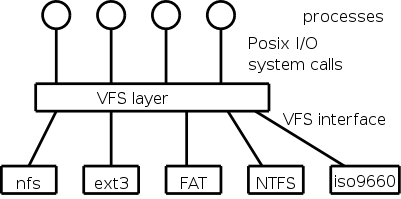
\includegraphics[scale=0.5]{vfs.png}
	\caption{Architektura Virtual File System}
    \label{fig:vfs}
\end{figure}

\section{File System in Userspace}
Do stworzenia QoSFS użyty zostanie moduł jądra, który umożliwia programowanie
logiki systemu plików - \textbf{FUSE (Filesystem in USErspace)}. 

\begin{figure}[h!]
	\centering
	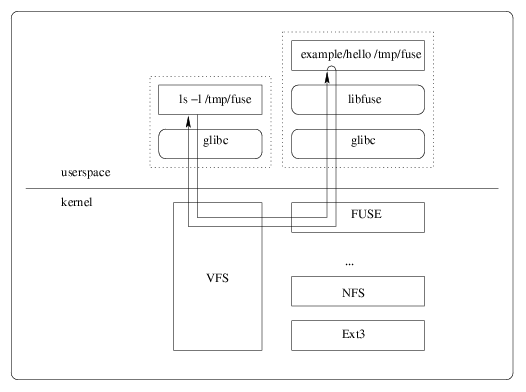
\includegraphics[scale=0.5]{fuse_structure.png}
		\caption{Struktura FUSE}
        \label{fig:fuse}
\end{figure}

Jest on szeroko znany i często używany
oraz stanowi bazę popularnego w GNU/Linux sterownika ntfs-3g\footnote{umożliwia
on dostęp odczytu/zapisu do systemu NTFS}.

Struktura FUSE przedstawiona została na rysunku \ref{fig:fuse}.

FUSE pozwala na programowanie w przestrzeni użytkownika, oraz konfigurację poprzez
pliki i aktualizację wersji bez restartu. 
Dzięki dostępowi do przestrzeni użytkownika będzie możliwe wykorzystanie standardowych
bibliotek bibliotek C.

\section{Flexible I/O tester}
Do testowania przepustowości użyte zostanie narzędzie \textbf{fio (flexible I/O tester)}.

Fio jest benchmarkiem wydajności I/O w systemach Unix, który pozwoli na
ocenienie poprawności zaproponowanego rozwiązania.

\chapter{Przegląd artykułów} \label{ch:articles}
W poniższym rodziale przedstawiono artukuły, które wykorzystane zostały
podczas pracy nad systemem.

\section{Providing Quality of Service in Object-Based File System}

Artykuł autorstwa Joela C. Wu, Scotta A. Brandta, powstał na \textit{University of California} w Santa Cruz.
Opisuje on framework \textbf{Bourbon}, który został zaprojektowany do pracy
z rozproszonym obiektowym systemem przechowywania danych \textbf{Ceph}\footnote{http://ceph.com/ceph-storage/file-system/}

Bourbon działa na podstawie wartości wagowych. Dzieli maksymalną przepustowość dysku
pomiędzy procesy i nadaje im maksymalną szybkość transferu danych bazując na 
nadanych wagach. Jeżeli proces A posiada wagę \texttt{.8} a proces B \texttt{.2}
to 80\% przepustowości zostanie przypisane procesowi A, a pozostałe 20\% procesowi B.

Do zapewnienia QoS Bourbon wykorzystuje istniejące już mechanizmy znajdujące sie 
w systemie plików EBOFS\footnote{Extended and B-tree based Object File System}, które
mogą być wykorzystane w Ceph.

Artykuł ten opisuje sposób buferowania zapytań I/O a w szczególności ich blokowania
w przypadku niedostepej przepustowości. Na tej podstawie zaprojektowano scheduler w QoSFS.

\section{Apollon: File System Level Support for QoS Augmented I/O}

Artykuł, którego autorami są: Taeseok Kim, Youjip Won, Doohan Kim, Kern Kohl i Yong H. Shin.
Opisuje system plików \textbf{Apollon}, którego celem jest obsługa odtwarzania
audio/wideo w czasie rzeczywistym jednocześnie np. z operacjami na bazie danych.

Stworzenie tego systemu było motywowane praktycznymi potrzebami obsłużenia standardów
\textbf{ATSC}\footnote{Advanced Television Systems Committee}(19.2 Mbits/s. dwe sesje odczytu i 
dwie zapisu) na urządzeniach PVR
\footnote{Personal Video Recorder}.

Apollon został zaprojektowany na wbudowane systemy z mała mocą obliczeniową.

W architekturze Apollon znajduje się Admission Controller,
którego zadaniem jest decydowanie o przyjęciu lub odrzuceniu zadań I/O oraz
Deadline-Driven I/O scheduler.

Mechanizm QoS klasyfukuje rodzaje operacji po rozszerzeniach plików i nadaje większy
priorytet tym z rozszerzeniami plików audio/video.

Na podstawie tego artykułu stworzono w QoSFS priorytetyzację procesów I/O
w zależności od typu pliku (nadano większy priorytet operacjom na plikach multimedialnych) oraz admission controller.

\section{Towards a QoS-aware Virtualised Storage System/Data Allocation Strategies for the Management of Quality of Service in Virtualised Storage Systems}

Oba artykuły zostały napisane przez Felipe Franciosi i Williama Knottenbelta. 
Skupiają się na
dostarczeniu mechanizmu QoS dla \textbf{VSS}\footnote{Virtualised Storage System}.

W pierwszym artykule opisano teoretyczne aspekty oraz przydatność
takiego mechanizmu a w drugim praktyczną implementacje i wyniki eksperymentów.

System dostarcza QoS poprzez
rozszerzenie standardowego systemu plików \textbf{ext3}\footnote{Third Extended File System} nazwanego \textbf{ext3ipods}. Realizowane jest to poprzez stworzenie dodatkowego i-węzła co pozwala na uzywanie
narzędzi takich jak \texttt{chattr} i \texttt{lsattr}.

Powyższy artykuł był inspiracją do uzycia i-węzłów do przechowywania metryk QoS, lecz pomysł został porzucony ze względu na brak potrzeby 
ustalania osobnych limitow dla każdego pliku.

\section{Provision of Storage QoS in Distributed File Systems for Clouds}

Artykuł napisany przez Chien-Min Wanga, Tse-Chen Yeha i Guo-Fu Tsenga skupia sie na dostarczeniu mechanizmu QoS dla obliczeń w chmurze. Projektowany system plików jest rozproszony
i oparty na modelu \textbf{ECNP}\footnote{Extended Contract Net Protocol}.

Architektura systemu jest modularna i składa się z Distributed FileSystem Client (DFSC) - odpowiedzialnego za przetwarzanie zapytań, 
z Metadata Manager (MM) - odpowiedzialnego za utrzymywanie globalnej listy zasobów,
i z Resource manager(RM) - pobierającego informacje w czasie rzeczywistym (np o aktualnej dostępnej szybkości transferu) i rejestrującego zasoby do MM.

Do zapewnienia QoS użyto \textbf{cgroups}, a dokładniej jego podmoduł \textbf{cgroups-blkio},
odpowiedzialnego za zarządzanie grupami kontrolnymi w ramach urządzeń I/O.

Na podstawie tego artykułu powstała wstępna architektura QoSFS (moduł główny, admission controller, scheduler) oraz odpowiedzialności każdego z modułów. Dodatkowo
postanowiono przetestować przydatność narzędzia \textbf{cgroups}.

\section{Quality of Service Support for Real-time Storage Systems}

Artykuł napisany przez Zorana Dimitrijevića i Raju Rangaswamiego.
Porusza on kwestię dostarczania mechanizmu QoS dla systemów czasu rzeczywistego.
Głownym celem jest ulepszenie działania aplikacji \textbf{VOD}\footnote{Video-on-Demand},
aplikacji \textbf{CCTV}\footnote{Close-circuit Television}, elektronicznych bibliotek,
\textbf{Virtual Reality} i różnych aplikacji naukowych potrzebujacych
dużej szybkości transferu danych.

W artykule opisano schedulery dysku (\textit{Deadline-based} oraz \textit{Cycle-based}) i sposób koltroli dostępu do zasobów (\textit{Best effort}, \textit{Deterministic} i \textit{Statistical}).
Zwrócono również uwagę na fizyczne ułożenie danych na dysku  -fragmentacja danych.
Położenie części pliku bliżej siebie na tarczy dysku
ograniczy dystans jaki pokona igła podczas operacji I/O.
Rozwiązanie to było rozważane w QoSFS, ale nie zostało zrealizowane
ponieważ alokacja plików na dysku w \textit{ext2} i \textit{ext3}
jest wystarczająca i defragmentacja nie jest wymagana.

Jako metodę dostarczania QoS podano i opisano schedulery: 
\begin{itemize}
	\item Kernel-Level scheduler
    \item Data-meta scheduler
    \item User-Level scheduler
\end{itemize}

Na podstawie tego artykułu przetestowano schedulery wbudowane w 
kernel Linuxa oraz zaprojektowano własny Data-meta scheduler.
